\documentclass{article}
\usepackage{iclr2027_conference}
\usepackage{amsmath,graphicx}
% The repository latexmk configuration uses XeLaTeX.  CJKutf8 is a
% pdfLaTeX-only interface and silently drops Chinese characters under XeLaTeX;
% ctex/xeCJK handles Unicode Chinese text and PDF metadata correctly.
\usepackage[UTF8,scheme=plain,fontset=none]{ctex}
\usepackage{fontspec}
\setmainfont{texgyretermes-regular.otf}[
  BoldFont=texgyretermes-bold.otf,
  ItalicFont=texgyretermes-italic.otf,
  BoldItalicFont=texgyretermes-bolditalic.otf]
\setsansfont{texgyreheros-regular.otf}[
  BoldFont=texgyreheros-bold.otf,
  ItalicFont=texgyreheros-italic.otf,
  BoldItalicFont=texgyreheros-bolditalic.otf]
\setCJKmainfont{Noto Serif CJK SC}[
  Script=CJK,Language=Chinese Simplified,AutoFakeSlant=.15]
\setCJKsansfont{Noto Sans CJK SC}[
  Script=CJK,Language=Chinese Simplified,AutoFakeSlant=.15]
\usepackage{booktabs,tabularx,array}
\usepackage{xcolor,tikz,etoolbox}
\usetikzlibrary{arrows.meta,positioning}
\usepackage[unicode,hidelinks]{hyperref}
\hypersetup{pdftitle={SURE-Evolve: Speech Model Research and Evaluation},
  pdfauthor={Anonymous authors},pdfsubject={ICLR 2027 manuscript}}
\newcommand{\pending}[1]{\textcolor{blue!65!black}{【待填：#1】}}
\newcommand{\resultcell}{\textcolor{blue!65!black}{待填}}
\newcolumntype{Y}{>{\raggedright\arraybackslash}X}
\newenvironment{keywords}{\vspace{.5em}\noindent\textbf{关键词}：}{\par}
\makeatletter
\def\fnum@figure{{\bf 图\ \thefigure}}
\def\fnum@table{{\bf 表\ \thetable}}
\makeatother

\title{SURE-Evolve：文献驱动的语音模型自动研究与统一评测}

\author{Anonymous authors}

\begin{document}
\maketitle
\raggedbottom

\begin{abstract}
语音模型的自进化需要有效利用已有研究，并依据可靠的实验反馈持续改进。
本文提出 SURE-Evolve，一个面向语音模型、融合文献知识与公平评测的自进化框架。
框架将大规模语音研究文献转化为关联研究问题与方法的知识图谱，以及可检索的方法组件库，支持面向具体问题提出模型改进方案。
框架自动实现候选方案并开展实验，在可比的模型执行条件与统一评分标准下对候选进行公平评测，为判断改进效果提供可靠依据。
框架结合文献先验与实验反馈积累研究经验，持续调整研究方向与修订候选方案，形成自进化闭环。
我们以自动语音识别（ASR）、语音合成（TTS）和说话人日志化（SD）为代表性任务，评估框架的自动研究能力及其对模型性能的改进效果。
\pending{正式结果：填写 ASR WER、TTS CER 和 SD DER
相对同协议基线的变化，并据此完成结论句。}
\end{abstract}

\begin{keywords}
自动化研究，语音处理，文献驱动智能体，模型优化，统一评测
\end{keywords}

\section{引言}
\label{sec:intro}

自动科研旨在让计算系统参与研究中的连续活动，包括理解已有知识、提出可检验的假设、
设计并执行实验、分析证据，以及依据结果修订研究方向。大语言模型已经使这些活动的
部分环节能够自动化\citep{lu2024aiscientist}，但面向语音模型的自动研究还需要处理领域
特有的研究对象、预测产物和评价条件。本文将 SURE-Evolve 定位为语音领域自动研究的
具体化：核心不在于重复一个与任务无关的智能体循环，而在于建立能够支撑语音研究闭环
的领域知识接口和实验反馈接口。

第一个接口是语音文献的收集与处理。ASR、TTS 和 SD 的研究文献数量大、方法描述涉及
不同的模型结构和实验条件，论文中的方法不能通过简单检索直接变成可执行的候选。要让
文献真正参与研究，需要从中整理研究问题、方法机制、适用条件和局限性，保留原文证据，
并将这些信息与当前任务、模型家族和允许的改动联系起来。SURE-Evolve 因此为三个语音
任务分别建立大规模、可检索和可追溯的知识基础，将文献内容转化为能够支持研究假设和
候选规格的领域证据。

第二个接口是语音任务的统一评测。语音研究的候选输出具有不同形式：ASR 产生转写文本，
TTS 产生合成波形，SD 产生带有说话人身份和时间边界的标注。它们分别涉及文本归一化、
音频转写后端以及 UEM、collar 和时间区间聚合等评分条件。SURE-Evolve 采用统一的评测
组织方式，同时保留每个任务的指标和协议：固定数据划分、产物格式、评分后端和聚合规则，
并记录实际使用的模型、配置和评测报告。这样得到的反馈既能反映任务性能，也能区分产物
缺失、执行失败和有效的模型改动，为跨轮候选比较提供可追溯的证据。

基于这两个接口，本文提出 SURE-Evolve，一个面向语音模型的文献驱动自动研究框架。框架
从语音文献、任务约束、当前最佳方案和历史实验出发，生成带有研究假设、作用机制和具体
改动的候选；候选由代码智能体实现，并在固定的执行条件下训练和推理；转写文本、合成
音频或说话人标注由 SURE~Eval 按任务协议检查和评分。性能、执行状态和预测产物随后写入
研究历史，用于调整下一轮研究方向，形成“文献证据—研究方案—候选实现—任务评测—
反馈修订”的闭环。我们以自动语音识别（ASR）、语音合成（TTS）和说话人日志化（SD）
为代表性任务，考察这一流程在不同语音模型和预测产物上的适用性。

本文的主要工作包括三个方面：首先，收集 ASR、TTS 和 SD 各自超过一万篇研究论文，
提取研究问题、方法和局限，构建带有原文证据的语音领域知识基础；其次，建立面向文本、
波形和时间标注的统一评测流程，在统一组织下保留各任务的评分协议，并将执行状态和
评测产物纳入研究反馈；最后，在 ASR、TTS 和 SD 三类任务上验证从文献检索、候选实现
到模型选择和独立评测的完整流程，分析其自动研究能力及适用范围。

\section{相关工作}
\label{sec:related}

\textbf{自动化研究与文献利用。}
The AI Scientist 将研究想法生成、实验实施和论文撰写组织为自动化流程，
展示了语言模型参与自动化研究的可能性\citep{lu2024aiscientist}。
检索增强生成将外部知识检索与文本生成结合，为研究过程中调用文献提供了
通用技术基础\citep{lewis2020rag}。本文在这些研究方向的基础上，聚焦语音
模型的实际改进。语音研究需要将方法描述落实为模型及其训练、推理流程的改动，
并处理转写文本、合成音频及说话人时间标注等不同预测产物。评测还涉及文本
归一化、音频转写后端和说话人计分边界等任务条件。我们围绕这些需求建立
文献驱动的方案生成、受控实验执行与统一评测流程，使研究假设能够接受语音
任务指标的实际检验。

\textbf{语音模型与任务差异。}
Zipformer 通过多时间分辨率编码器等设计进行语音识别\citep{yao2024zipformer}；
F5-TTS 基于流匹配进行语音生成\citep{chen2024f5tts}；DiariZen 所采用的
自监督语音表示与日志化网络支持说话人活动建模\citep{han2025leveraging}。
这些模型提供了不同的结构改进空间，也对应不同的输出形式。我们以它们为
实例，保留各模型家族的任务特性，通过任务定义、候选执行接口和 SURE~Eval
评测管理组织实验。框架以任务定义描述输入输出、允许的模型改动和评价目标，
由执行接口适配具体模型的训练与推理过程，使不同语音任务能够沿用同一研究
流程，并保留自身的数据与评价指标。

\section{SURE-Evolve 框架}
\label{sec:method}

\subsection{问题定义与研究闭环}

我们将语音模型的自进化视为由领域知识与实验观察共同驱动的方案搜索。
对于任务 $\tau$，候选方案 $c$ 描述模型及其训练、推理方法。框架从初始
方案 $c_0$ 出发，利用文献集合 $\mathcal{P}_{\tau}$ 形成研究假设，再通过
真实实验更新对候选的判断。方案生成由当前研究问题引导，可涉及模型结构、
训练方法或推理策略；实验条件 $\mathcal{C}_{\tau}$ 则提供可比的验证基准。
图~\ref{fig:framework} 展示了这一过程在不同语音任务中的统一组织方式。

\begin{figure}[t]
\centering
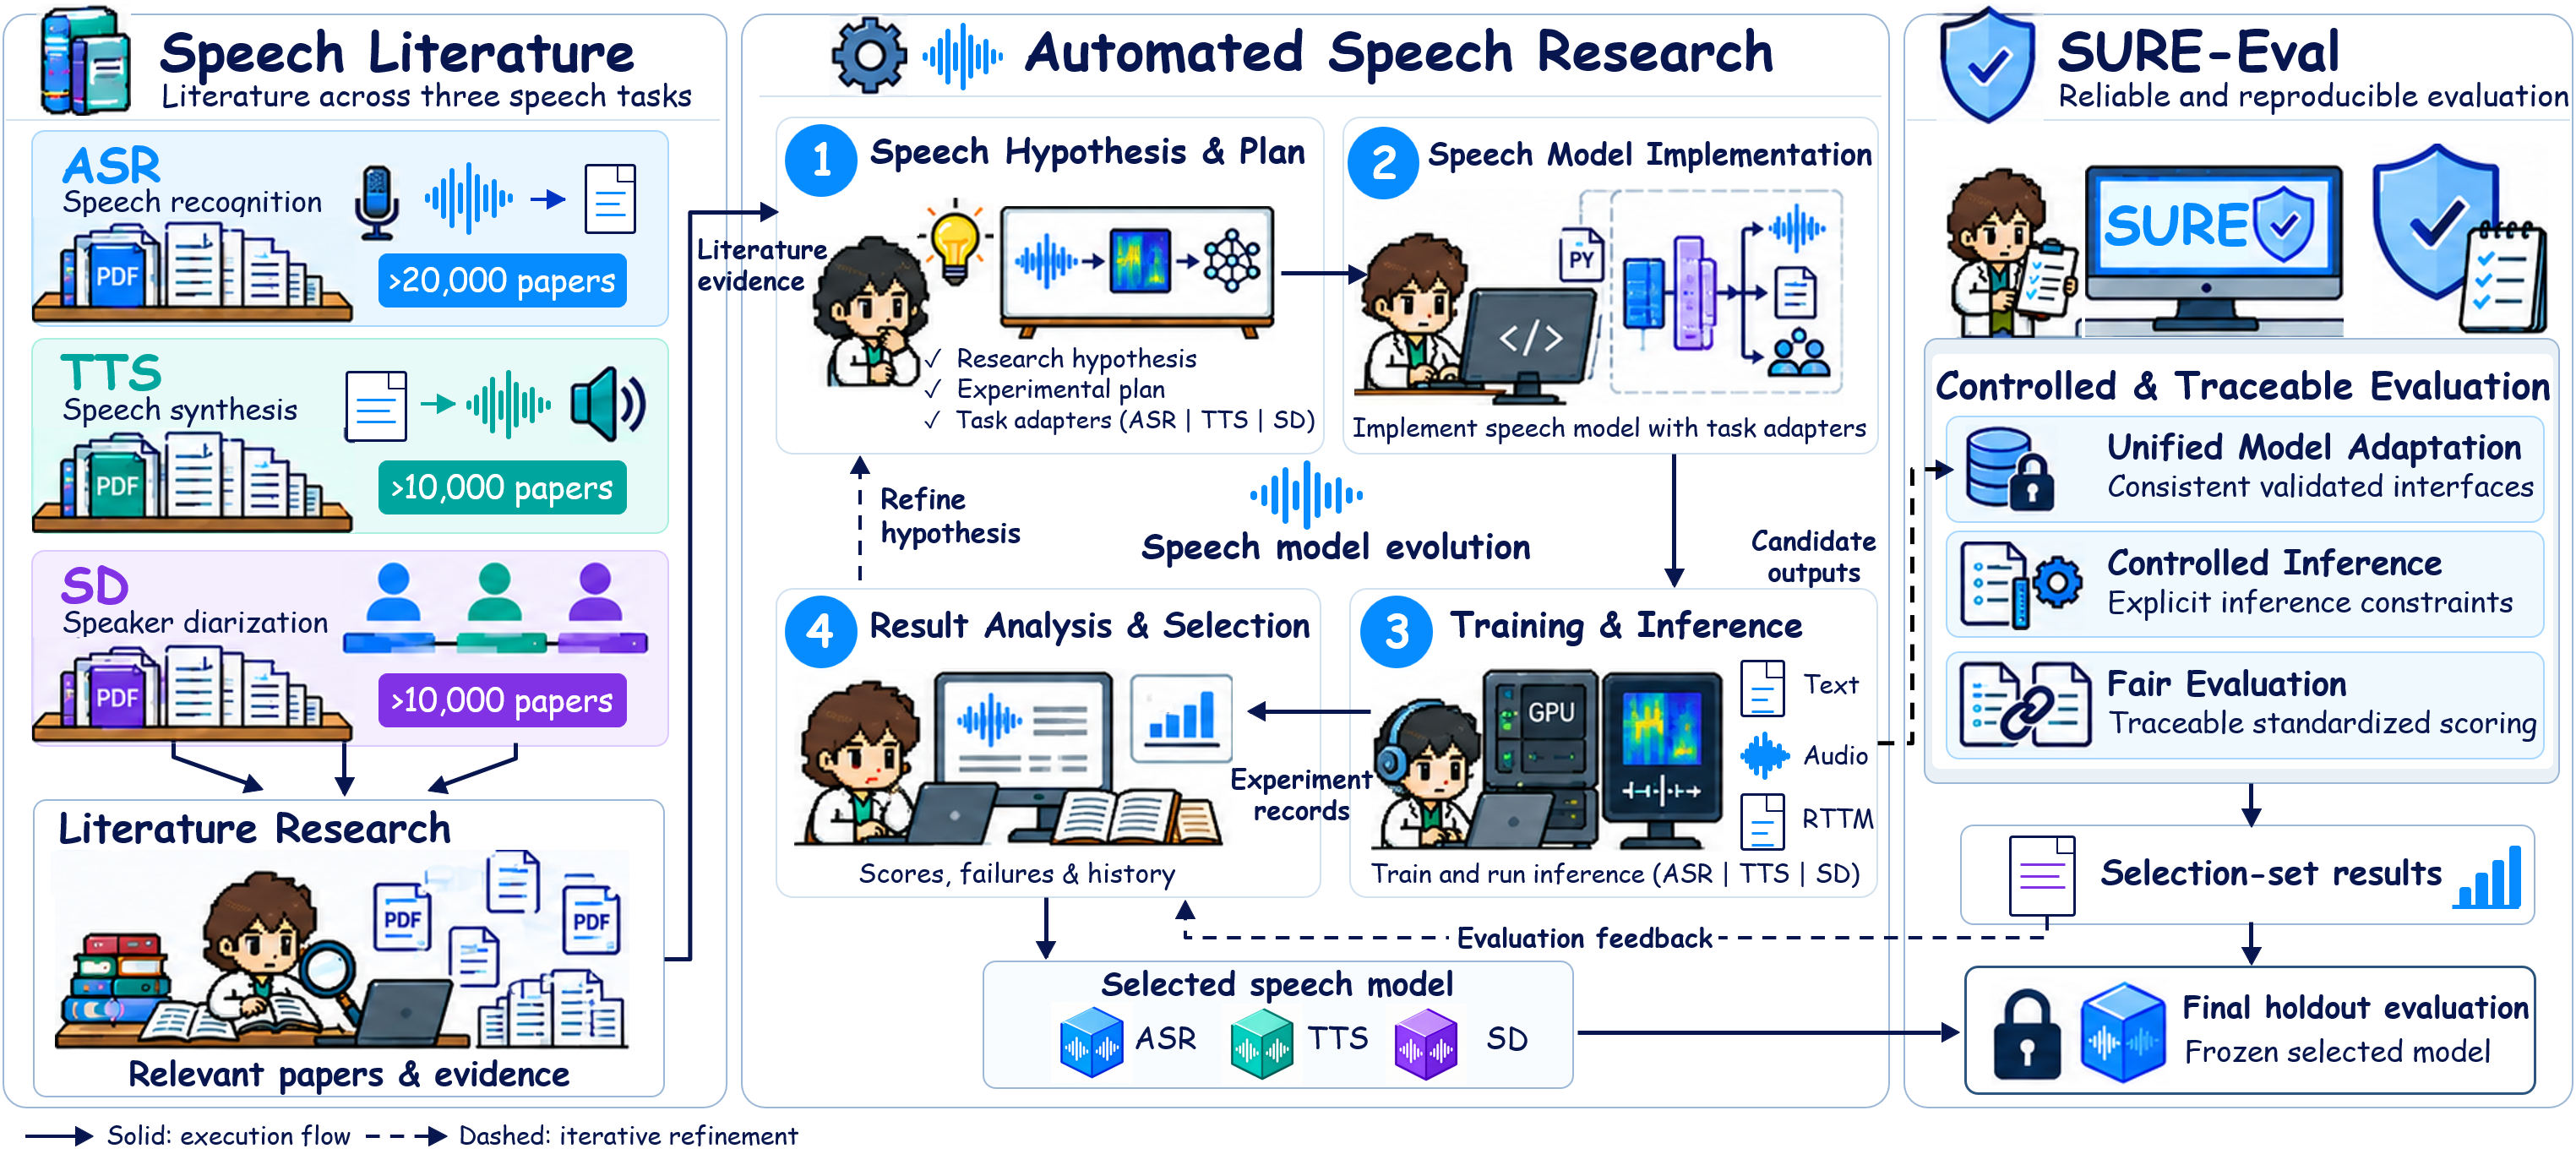
\includegraphics[width=\linewidth]{framework.png}
\caption{SURE-Evolve 面向语音场景的研究闭环，以 ASR、TTS 和 SD 为例。
上方为搜索阶段，反馈来自实际实验；下方为搜索结束后的模型选择与最终评测，
保留测试集结果不进入后续研究反馈。}
\label{fig:framework}
\end{figure}

闭环的核心是研究假设与实验反馈的相互作用。文献为候选提供方法依据，历史
实验则揭示这些思路在当前语音任务中的适用性。每轮研究据此形成一组候选，
其实际表现经 SURE~Eval 转化为后续推理的依据。候选实现、预测产物与评分
之间的对应关系，使跨轮研究能够建立在已经观察到的结果之上。

\subsection{语音文献驱动的研究方案生成}

我们收集了 ASR、TTS 和 SD 各自超过一万篇的研究论文，提取研究问题、
核心方法与局限性，构建知识图谱和方法组件的向量索引，并保留原文证据。
这些结构化知识与文献综述共同支持面向当前研究问题的检索，为改进方案的
生成与比较提供可追溯的依据。

研究模块结合当前方案与历史实验分析改进方向，在文献证据支持下开展多种研究偏好下的方案搜索，并通过评议与融合形成候选。每个候选明确研究假设、作用机制和具体改
动，使文献中的方法能够转化为可执行、可检验的研究方案。

以 $\mathcal{H}_{t-1}$ 表示此前实验历史，第 $t$ 轮研究过程可记为
\begin{equation}
\mathcal{I}_t=\mathcal{R}_{\mathrm{speech}}
 (\mathcal{P}_{\tau},\mathcal{C}_{\tau},c^*_{t-1},\mathcal{H}_{t-1}),
\end{equation}
其中 $\mathcal{R}_{\mathrm{speech}}$ 表示语音研究方案生成过程，
$\mathcal{I}_t$ 为本轮候选方案集合，$c^*_{t-1}$ 为当前最佳方案。

\subsection{候选实现与控制变量实验}

候选进入实验前，框架结合任务条件审查其证据依据、执行可行性及与已有尝试的差异。通过审查的方案被转化为明确的修改规格，再由代码智能体完成实现。方案评议用于选择值得实验的候选，模型性能则由后续实测判断。

代码智能体将研究假设落实为模型代码或配置的修改，框架根据候选方案组织相应实验。为保证比较的可解释性，实验明确记录候选相对于参照方案的改动，并保持非干预条件可比。方案带来的模型规模、计算量和运行成本变化与性能一并报告。

实验生成任务所需的预测产物，并保留对应的模型与配置，使研究方案、实际实现和评测结果能够相互对应。这些产物由 SURE~Eval 统一评分，为后续候选比较和研究迭代提供依据。

\subsection{结果反馈与模型选择}

设 $\theta_{t,j}$ 为候选方案 $c_{t,j}$ 对应的模型参数，$F_{\tau}$ 为任务 $\tau$ 的推理过程，其行为由候选方案与模型参数共同确定。搜索阶段候选得分为
\begin{equation}
s_{t,j}=\operatorname{SURE\,Eval}_{\tau}
 \bigl(F_{\tau}(c_{t,j},\theta_{t,j};\mathcal{D}_{\mathrm{search}})\bigr).
\end{equation}
框架通过 SURE~Eval 统一评测候选方案，以各任务对应的误差率衡量其表现。框架将候选改动、实测得分与执行状态共同写入研究历史，供下一轮分析与方案生成使用。对于已有可继续改进的方案，
研究模块结合实验反馈重新分析其不足并修订研究方向；对于重复尝试，则要求说明新的实验条件或尚未解决的问题。执行失败与性能未改善分别记录，以免将环境或程序故障误
解为研究假设不成立。

搜索结束后，独立选择集用于在基线与入围候选之间确定最终方案。最终评价
使用保留测试集，并冻结各方案的模型权重与推理配置，以考察研究结果在
未参与迭代的数据上的表现。测试结果不再进入研究反馈。

\subsection{统一评测与实验可比性}
\label{sec:evaluation}

在自进化过程中，评测结果既决定当前候选的取舍，也作为历史证据指导下一轮研究。即使预测结果相同，文本归一化、评价后端或聚合方式的差异也可能改变分数；若候选之间或轮次之间的评分口径不一致，系统便可能把这种差异误判为模型改进，进而影响后续研究方向。因此，统一且可比的评测是形成可靠迭代反馈的基础。SURE~Eval 通过显式的
执行与评分协议，将模型输出、评分流程及其版本关联起来，为结果的公平比较与复核提供依据\citep{sureeval_manuscript}。

为此，本文对同一任务的基线与候选固定数据划分和评分链，将研究干预之外的执行条件作为控制变量，明确记录候选的模型与运行配置。候选程序只负责生成预测产
物，评分由框架统一调用预定义程序完成，候选代码不负责计分，也不允许修改评分实现。这一分工减少了评分口径变化对候选比较的影响，使性能差异能够在共同实验条件下解
释。

评测前，框架检查必需产物及任务对应的输出要求；产物缺失、校验不通过或评分失败的尝试不作为有效性能结果参与比较。每次评测保存实际使用的流水线、节点版本、输入文
件信息与评分报告，使得分能够追溯到相应预测及计算过程。不同任务保留各自的指标含义，同一任务的所有候选采用一致的评分协议：

\textbf{ASR。} 固定 Whisper 英语文本归一化与 WeNet 兼容评分实现，以 WER 比较识别结果，避免将文本处理规则的差异计入模型改
进。

\textbf{TTS。} 固定音频预处理、Paraformer 转写后端、标点处理与字符评分链，以 CER 评价合成语音的可懂度，减少评价用识别器差异的影
响。该指标不涵盖自然度与说话人相似度。

\textbf{SD。} 固定 DER 的计分边界与聚合规则，采用 $0.25$ 秒 collar，对参考与预测标注按 UEM 裁剪，并使用会话误差率的算术
平均，确保不同候选在相同计分口径下比较。

\pending{填写正式实验使用的 SURE~Eval 版本与评分节点配置，冻结 SD 重叠语音计分选项及后端版本；补充 SURE~Eval 原文的正式书
目信息。}

\section{实验与结果}
\label{sec:experiments}

\subsection{任务、模型与数据}

我们选择三种不同类型的语音任务作为框架的验证实例。ASR 使用 Zipformer 和 TED-LIUM 3
英语语音数据\citep{yao2024zipformer,hernandez2018tedlium}；TTS 使用
F5TTS\_v1\_Base，在 WenetSpeech4TTS-Premium 的训练划分上进行微调，
并保留 Seed-zh 作为最终测试数据\citep{chen2024f5tts,ma2024wenetspeech4tts}；
SD 使用 DiariZen 的 WavLM-updated 路线，在 AMI 单通道会议语音上训练
和评测\citep{han2025leveraging,carletta2006ami}。各任务的文献规模与
实验对象概括于表~\ref{tab:tasks}。

\begin{table}[t]
\centering
\caption{领域文献与语音实验对象。文献规模为各领域独立计数。}
\label{tab:tasks}
\setlength{\tabcolsep}{4pt}
\begin{tabularx}{\columnwidth}{l c Y}
\toprule
任务 & 文献数量 & 基础模型与主要数据 \\
\midrule
ASR & $>10{,}000$ & Zipformer；TED-LIUM 3 \\
TTS & $>10{,}000$ & F5-TTS；WenetSpeech4TTS-Premium、Seed-zh \\
SD & $>10{,}000$ & DiariZen；AMI \\
\bottomrule
\end{tabularx}
\end{table}

ASR 的搜索和选择数据由开发数据按演讲分组划分，官方测试数据仅用于
最终评测。TTS 的训练与开发划分按原始录音分组，固定参考语音、参考文本
和目标文本。SD 按会议分组，统一输入通道和评测时间区域。
\pending{填写每个划分的样本数、时长与清单版本；补充 Seed-zh 数据来源引用。}

\subsection{基线与研究设置}

以下配置构成三个任务的基线配方。ASR 使用完整训练划分，从头训练
30 个 epoch，采用 RNN-T 目标、随机种子 42 和贪心解码。
TTS 从 F5-TTS 官方预训练权重初始化，使用 AdamW、学习率 $10^{-5}$、
随机种子 42，微调 100 个 epoch，最终采用 EMA 权重。SD 使用
WavLM-Base+ 自监督权重初始化主干，其余网络从头初始化；主干与其余网络
学习率分别为 $2\times10^{-5}$ 和 $10^{-3}$，随机种子为 3407，最多
训练 100 个 epoch，训练验证损失连续 10 次不改善时早停，并平均验证损失
最好的五个检查点。

基线采用 FP32 计算；TTS 的流匹配采样步数为 32，SD 使用 8 秒片段
及相应聚类配置。候选从研究问题出发提出改动，非干预条件沿用上述基准，
具体变化随最终方案报告。研究预算分别约束内部方案搜索与外部候选实验：前者控制方案探索、评议和生成尝试，后者控制研究轮数、进入实验的候选数及训练与推理资
源。\pending{核对正式基线配方，填写内部方案搜索策略及预算（包括 MCTS 迭代与评议预算）、每轮候选生成与审查的尝试上限、最终进入实验的候选数、研
究轮数与实验资源预算、研究及代码智能体的 LLM 配置，以及最终候选相对基线的改动。以上数值以正式运行配置为准。}

\subsection{对照与报告方式}

每个任务比较初始基线与 SURE-Evolve 最终选出的方案，在控制非干预条件
的基础上衡量整体改进。主结果取自保留测试集；搜索过程的分数用于描述开发集
上的研究轨迹。误差率相对变化定义为
\begin{equation}
\Delta_{\mathrm{rel}}=
\frac{e_{\mathrm{base}}-e_{\mathrm{final}}}{e_{\mathrm{base}}}\times100\%,
\end{equation}
其中 $e_{\mathrm{base}}>0$。正值表示误差率下降，负值表示误差率上升。
同时保留原始误差率，以便区分绝对百分点变化和相对变化。
\pending{填写独立运行次数；如有重复实验，报告均值与标准差，并说明搜索与训练种子。}

\subsection{三个任务上的最终表现}
\label{sec:results}

表~\ref{tab:results} 给出最终测试结果的统一报告形式。每个任务先报告
基线与最终模型的绝对误差率，再给出相对变化。三个任务的指标分别解释，
以呈现同一研究流程在不同模型与数据条件下的完整系统表现。

\begin{table}[t]
\centering
\caption{保留测试集上的主结果。所有误差率以百分比表示；待填项将在正式
实验完成后补入。}
\label{tab:results}
\setlength{\tabcolsep}{3pt}
\begin{tabular*}{\columnwidth}{@{\extracolsep{\fill}}l l c c c@{}}
\toprule
任务 & 指标 $\downarrow$ & 基线 & 最终方案 & 相对变化 \\
\midrule
ASR & WER & \resultcell & \resultcell & \resultcell \\
TTS & CER & \resultcell & \resultcell & \resultcell \\
SD & DER & \resultcell & \resultcell & \resultcell \\
\bottomrule
\end{tabular*}
\end{table}

\pending{ASR 结果段：填写基线与最终方案的 WER、主要改动及模型或计算成本变化，
说明测试集与开发集表现的关系。}

\pending{TTS 结果段：填写 CER 的变化及最终方案，结论限定为合成语音的
可懂度；若补充相似度或听测，再分别描述这些维度的结果。}

\pending{SD 结果段：填写 DER 的变化及最终方案，并注明本表使用的 collar、
重叠处理和会话聚合协议；只有存在错误分解数据时才解释漏检、误检或混淆变化。}

\subsection{研究过程与实验成本}

研究过程以逐轮候选表现和历史最优轨迹呈现，结合实验成本描述最终方案的
获得过程。第~\ref{sec:case} 节进一步分析代表性候选的研究依据与语音机制。
\pending{补入真实运行的候选轨迹及关键改动，标注有效实验与失败尝试。}

实验成本以表~\ref{tab:cost} 汇总。方案生成尝试数与实际进入实验的候选数分别记录，实验候选同时报告尝试和成功数量。训练设备时包含失败尝试所消耗
的计算；LLM 用量覆盖方案搜索、评议、融合、候选审查、实现和调试阶段。
各模型的推理耗时在同任务、同硬件和同批处理设置下测量。设备时与实际
运行时间分别记录，以区分累计资源消耗和并行执行后的墙钟时间。
\pending{注明文献预处理成本是否计入总成本；若单独统计，补充其资源消耗及跨研究运行的复用方式。}

\begin{table}[t]
\centering
\caption{完整研究运行的规模与资源记录。不同任务的硬件型号另行注明，
不直接将异构设备时解释为等价计算量。}
\label{tab:cost}
\setlength{\tabcolsep}{3pt}
\begin{tabularx}{\columnwidth}{Y c c c}
\toprule
记录项 & ASR & TTS & SD \\
\midrule
研究轮数 & \resultcell & \resultcell & \resultcell \\
方案生成尝试数 & \resultcell & \resultcell & \resultcell \\
实验候选数（尝试/成功） & \resultcell & \resultcell & \resultcell \\
训练设备时（小时） & \resultcell & \resultcell & \resultcell \\
LLM 用量（百万 token） & \resultcell & \resultcell & \resultcell \\
总运行时间（小时） & \resultcell & \resultcell & \resultcell \\
\bottomrule
\end{tabularx}
\end{table}

\subsection{讨论}

本文的实验评价完整研究流程在给定数据与资源条件下获得的最终方案。
开放的方案生成可能同时涉及多项相关改动，因此整体性能变化与某一模块
的独立作用需要区分。候选引入的模型规模、训练成本和推理开销也应纳入
结果解释。TTS 的自动转写误差率主要反映可懂度，后续可结合自然度与
说话人保持评价扩展质量分析。

\section{案例分析：候选方案的语音机制}
\label{sec:case}

本节围绕一个代表性候选，沿“文献依据—研究假设—实际改动—实验观察—后续修订”的过程，分析其形成与演进，建立自动研究过程与语音建模问题之间的联系。

\subsection{研究假设与候选方案}

\pending{选定一个真实候选，交代目标语音任务与基线面临的问题，利用已有文献证据和候选记录说明研究假设如何形成，以及如何落实为实际改动。}

\subsection{语音理论与作用机制}

\pending{选择与实际候选直接相关的语音理论，建立“具体改动—作用机制—
预期现象”的解释。结合模型结构图、必要公式或文献说明其可能有效的原因。}

\subsection{实验观察与适用范围}

\pending{结合该候选与基线的已有实验结果、代表性语音样例或错误分布，讨论观测是否与机制解释一致，并说明适用条件。依据已有研究记录说明反馈如何影响后续修订；若无后续尝试，则明确说明。将实测结果与尚待验证的解释区分。}

\section{结论}
\label{sec:conclusion}

本文提出面向语音场景的自动研究框架 SURE-Evolve，以 ASR、TTS 和 SD
为代表性实例，收集各自超过一万篇的研究论文，建立了从文献分析、模型改进
假设、实验执行到 SURE~Eval 反馈的迭代闭环。框架以文献和实验观察引导
研究方向，通过控制非干预条件比较候选，并在独立数据上评价最终方案。
三个任务的实验与代表性候选分析共同呈现该流程在语音模型研发中的表现。
\pending{依据表~\ref{tab:results} 填写最终结论：明确哪些任务取得提升、
幅度及对应成本；不预设所有任务提升或达到最优水平。}

\clearpage
\begingroup
\interlinepenalty=10000
\bibliographystyle{iclr2027_conference}
\bibliography{sure_evolve_refs}
\endgroup
\end{document}
